\documentclass{article}

\usepackage[T2A]{fontenc}
\usepackage[utf8]{inputenc}
\usepackage[russian]{babel}

\usepackage[unicode, colorlinks, linkcolor=blue]{hyperref}

\usepackage{graphicx}
\graphicspath{{pictures/}}
\DeclareGraphicsExtensions{.pdf,.png,.jpg}

\usepackage{pgfplots}
\usepackage{tikz}

\usepackage{comment}

\begin{document}
\selectlanguage{russian}
	%----------------------------------Шапка------------------------------------
\begin{center}
	
\includegraphics[scale=0.25]{AU}\\
	{\Large\bfseries Санкт-Петербургский национальный исследовательский Академический университет имени Ж.И.~Алфёрова Российской академии наук}
\end{center}

\begin{center}
	{\large\textbf{Рабочий протокол и отчёт по лабораторной работе № 8}}\\
	Свиридов Фёдор, Александр Слободнюк, Владимир Попов
\end{center}

\begin{center}
	\rule{12cm}{0.4mm}\\
	\large\bfseries{<<Измерение энтропии>>}\\
	\rule{12cm}{0.4mm}
\end{center}
%-----------------------------------------------------------------------------
 \paragraph{Рабочие формулы и исходные данные.}
 

 	\begin{figure}[htb]
 		\caption{}
 		 \begin{center}
 	 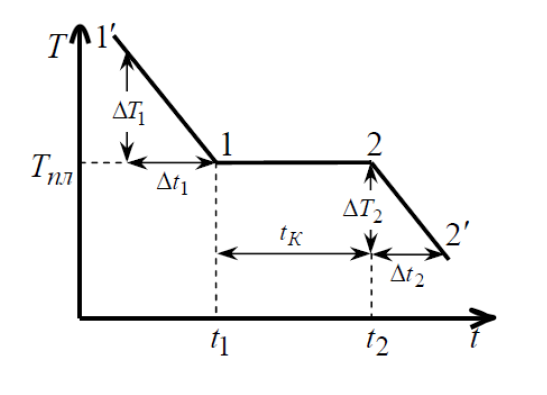
\includegraphics[scale=0.3]{plot}
 	   \end{center}
 	\end{figure}


 В опыте используется сплав массой $ M_0=120\;\mbox{г.}$ , который состоит из 60 \% олова и 40 \% свинца. Также в процессе теплообмена участвует стальная  ампула массой $ M_a = 500\;\mbox{г.}$ Удельные теплоёмкости данных материалов:
 
 $ C_a\mbox{(сталь)} = 460\; \frac{\mbox{Дж}}{\mbox{кг} \cdot \mbox{К}}$
 
 $ C_{Sn} = 228\; \frac{\mbox{Дж}}{\mbox{кг} \cdot \mbox{К}}$
 
 $ C_{Pb} = 128\; \frac{\mbox{Дж}}{\mbox{кг} \cdot \mbox{К}}$
 
 Следовательно, удельная теплоёмкость сплава:
 
 $ C_0 = 0,6\,C_{Sn}+0,4\,C_{Pb} = 188\; \frac{\mbox{Дж}}{\mbox{кг} \cdot \mbox{К}}$\\
 
  Изменение энтропии:
 \begin{equation}
 	S_2-S_1=\frac{\lambda M_0}{T}
 \end{equation}

 Удельная теплота кристаллизации сплава:
 \begin{equation}
 	\lambda=\frac{C_0M_0+C_aM_a}{M_0}\;\frac{\Delta T}{\Delta t}\;\Delta t_k
 \end{equation}
, где $ \frac{\Delta T}{\Delta t}\;\Delta t_k $ средняя скорость остывания сплава на участках \\
$ 1^{'}\rightarrow1 $ и $ 2\rightarrow2^{'} $(Рис. 1); $ \Delta t_k $ - время кристаллизации сплава

\paragraph{Результаты прямых измерений и их обработки.}
Результаты прямых измерений в \hyperlink{table}{приложении}.\\
 \begin{tikzpicture}
 	\begin{axis}[nodes near coords,enlargelimits=0.2,xlabel={Время $t$, c}, ylabel={Температура $ T{,}\;^{\circ}$C}]
 		\addplot+[black, point meta=explicit symbolic, mark size=1pt, only marks] 
 		coordinates {
 			(	0	,	191.6	)[$1^{'}  $]
 			(	20	,	190.0	)
 			(	40	,	188.0	)
 			(	60	,	186.1	)
 			(	80	,	184.0	)
 			(	100	,	181.9	)
 			(	120	,	180.2	)
 			(	140	,	178.5	)
 			(	160	,	177.0	)
 			(	180	,	176.3	)
 			(	200	,	176.1	) [1]
 			(	220	,	176.1	)
 			(	240	,	176.6	)
 			(	260	,	176.8	)
 			(	280	,	176.8	)
 			(	300	,	176.8	)
 			(	320	,	176.6	)
 			(	340	,	176.4	)
 			(	360	,	176.2	)
 			(	380	,	176.1	)
 			(	400	,	175.9	)
 			(	420	,	175.7	)
 			(	440	,	175.6	)
 			(	460	,	175.4	)
 			(	480	,	175.3	)
 			(	500	,	175.3	)
 			(	520	,	175.2	)
 			(	540	,	175.2	)
 			(	560	,	175.2	)
 			(	580	,	175.1	)
 			(	600	,	175.1	)
 			(	620	,	175.1	)
 			(	640	,	175.1	)
 			(	660	,	175.0	)
 			(	680	,	175.0	)
 			(	700	,	174.9	)
 			(	720	,	174.8	)
 			(	740	,	174.8	)
 			(	760	,	174.8	)
 			(	780	,	174.7	)
 			(	800	,	174.7	)
 			(	820	,	174.6	)
 			(	840	,	174.5	)
 			(	860	,	174.4	)
 			(	880	,	174.3	)
 			(	900	,	174.2	)
 			(	920	,	174.1	)
 			(	940	,	174.0	)
 			(	960	,	173.9	)
 			(	980	,	173.8	)
 			(	1000	,	173.7	)
 			(	1020	,	173.6	)
 			(	1040	,	173.5	)
 			(	1060	,	173.3	)
 			(	1080	,	173.2	)
 			(	1100	,	173.0	)
 			(	1120	,	172.7	)
 			(	1140	,	172.4	)
 			(	1160	,	172.1	)[$ \;2 $]
 			(	1180	,	170.7	)
 			(	1200	,	169.1	)
 			(	1220	,	167.0	)
 			(	1240	,	164.6	)
 			(	1260	,	162.4	)
 			(	1280	,	160.5	)
 			(	1300	,	158.7	)
 			(	1320	,	156.7	)
 			(	1340	,	155.1	)
 			(	1360	,	153.6	)
 			(	1380	,	151.7	)
 			(	1400	,	150.3	)
 			(	1420	,	148.7	)
 			(	1440	,	147.0	)
 			(	1460	,	145.9	)
 			(	1480	,	144.2	)
 			(	1500	,	143.1	)
 			(	1520	,	141.9	)
 			(	1540	,	140.6	)
 			(	1560	,	139.2	)
 			(	1580	,	138.0	)
 			(	1600	,	136.6	)
 			(	1620	,	135.4	)
 			(	1640	,	134.2	)
 			(	1660	,	133.0	)
 			(	1680	,	131.7	)
 			(	1700	,	130.4	)
 			(	1720	,	129.1	)
 			(	1740	,	128.0	)
 			(	1760	,	126.9	)
 			(	1780	,	125.7	)
 			(	1800	,	124.5	)
 			(	1820	,	123.4	)
 			(	1840	,	122.2	)
 			(	1860	,	120.9	)
 			(	1880	,	120.0	)
 			(	1900	,	118.8	)
 			(	1920	,	117.7	)
 			(	1940	,	116.6	)[	$\;2^{'}  $]
 		};
 	\end{axis}
 \end{tikzpicture}



\begin{table}
	\centering {\large\bfseries Приложение}\hypertarget{table}{}\\
	\caption{Зависимость температуры от времени}
	\begin{tabular}{cc||cc||cc||cc}
		t, c& T, $ ^\circ C $&t, c& T, $ ^\circ C $&t, c& T, $ ^\circ C $&t, c& T, $ ^\circ C $\\
		\hline
		0	&	191.6	&	500	&	175.3	&	1000	&	173.7	&	1500	&	143.1	\\
		20	&	190.0	&	520	&	175.2	&	1020	&	173.6	&	1520	&	141.9	\\
		40	&	188.0	&	540	&	175.2	&	1040	&	173.5	&	1540	&	140.6	\\
		60	&	186.1	&	560	&	175.2	&	1060	&	173.3	&	1560	&	139.2	\\
		80	&	184.0	&	580	&	175.1	&	1080	&	173.2	&	1580	&	138.0	\\
		100	&	181.9	&	600	&	175.1	&	1100	&	173.0	&	1600	&	136.6	\\
		120	&	180.2	&	620	&	175.1	&	1120	&	172.7	&	1620	&	135.4	\\
		140	&	178.5	&	640	&	175.1	&	1140	&	172.4	&	1640	&	134.2	\\
		160	&	177.0	&	660	&	175.0	&	1160	&	172.1	&	1660	&	133.0	\\
		180	&	176.3	&	680	&	175.0	&	1180	&	170.7	&	1680	&	131.7	\\
		200	&	176.1	&	700	&	174.9	&	1200	&	169.1	&	1700	&	130.4	\\
		220	&	176.1	&	720	&	174.8	&	1220	&	167.0	&	1720	&	129.1	\\
		240	&	176.6	&	740	&	174.8	&	1240	&	164.6	&	1740	&	128.0	\\
		260	&	176.8	&	760	&	174.8	&	1260	&	162.4	&	1760	&	126.9	\\
		280	&	176.8	&	780	&	174.7	&	1280	&	160.5	&	1780	&	125.7	\\
		300	&	176.8	&	800	&	174.7	&	1300	&	158.7	&	1800	&	124.5	\\
		320	&	176.6	&	820	&	174.6	&	1320	&	156.7	&	1820	&	123.4	\\
		340	&	176.4	&	840	&	174.5	&	1340	&	155.1	&	1840	&	122.2	\\
		360	&	176.2	&	860	&	174.4	&	1360	&	153.6	&	1860	&	120.9	\\
		380	&	176.1	&	880	&	174.3	&	1380	&	151.7	&	1880	&	120.0	\\
		400	&	175.9	&	900	&	174.2	&	1400	&	150.3	&	1900	&	118.8	\\
		420	&	175.7	&	920	&	174.1	&	1420	&	148.7	&	1920	&	117.7	\\
		440	&	175.6	&	940	&	174.0	&	1440	&	147.0	&	1940	&	116.6	\\
		460	&	175.4	&	960	&	173.9	&	1460	&	145.9	&		&		\\
		480	&	175.3	&	980	&	173.8	&	1480	&	144.2	&		&		
	\end{tabular}
\end{table}

\end{document}
